\section{Test concorrenziale con IO}

Nel seguente test si vuole testare la concorrenza
come nel test del paragrafo \ref{sec:test_concorrenziale}
ma invece di variare il numero di prodotti per ogni
processo, si varia il numero di operazioni di Input
ed Output su File. Queste operazioni impiegano più tempo
rispetto ai prodotti, quindi ci si aspetta di mettere
maggiormente in evidenza il guadagno che si ha nell'usare più
processi rispetto all'utilizzarne uno solo.

%++++++++++++++++++++++++++++++++++++++++++++++
\subsection{Implementazione del test}

Il codice Elixir che esegue il test è
implementato nel modulo Elixir TaskIO e
riportato nel Listing \ref{lst:concurrent_task_io}.


\begin{lstlisting}[language=elixir, caption={Test concorrenziali},captionpos=b,
	label={lst:concurrent_task_io}]

defmodule TaskIO do
	require Logger
  
	import MyFile
  
	# decodifica del file Json
	def parse_json_file(file_path \\ "./File/read.json") do
	  case File.read(file_path) do
		{:ok, json_data} ->
		  case Poison.decode(json_data) do
			{:ok, parsed_json} ->
			  parsed_json
  
			{:error, reason} ->
			  IO.puts("Failed to parse JSON: #{reason}")
			  nil
		  end
  
		{:error, reason} ->
		  IO.puts("Failed to read file: #{reason}")
		  nil
	  end
	end
  
	# caso base ricorsione
	def compute_products(0, _file) do
	  nil
	end
  
	def compute_products(operations, file) do
	  data = parse_json_file()
  
	  # calcolo risultati del json
	  somma = data["somma"] |> Enum.reduce(fn x, acc -> acc + x end)

	  sottrazione = data["sottrazione"] 
	  |> Enum.reduce(fn x, acc -> acc - x end)

	  moltiplicazione = data["moltiplicazione"] 
	  |> Enum.reduce(fn x, acc -> acc * x end)

	  divisione = data["divisione"] 
	  |> Enum.reduce(fn x, acc -> acc / x end)
  
	  # scrittura risultati del nel file csv
	  result = [
		"#{somma},",
		"#{sottrazione},",
		"#{moltiplicazione},",
		"#{divisione}\n"
	  ]
  
	  IO.write(file, result)

	  # chiamata ricorsiva
	  compute_products(operations - 1, file)
	end
  
	def run do
	  processes = [1, 2, 3, 4, 5, 6, 7, 8, 16, 32, 64, 128, 256, 512]
	  operationsnumber = 20_000
	  step = 250
  
	  {:ok, file} = File.open("./File/write.csv", [:write, :append])
  
	  for proc <- processes do
		for comp <- 500..operationsnumber//step do
		  {:ok, _time} = parallel_operations(comp, proc, file)
		end
	  end
  
	  File.close(file)
	end
  
	def parallel_operations(operationsnumber, processnumber, file) do

	  # calcolo del numero di operazioni da dare ad ogni processo
	  temp = trunc(operationsnumber / processnumber)

	  # calcolo del resto 
	  rest = rem(operationsnumber, processnumber)
  
	  {time, _result} =
		:timer.tc(
		  fn ->
			tasks =
			  for _i <- 1..processnumber do
				Task.async(fn -> compute_products(temp, file) end)
			  end
  
			restTask = Task.async(fn -> compute_products(rest, file) end)
  
			# Per ogni task aspetta di finire
			for task <- tasks do
			  Task.await(task, :infinity)
			end
  
			Task.await(restTask, :infinity)
		  end,
		  [],
		  :microsecond
		)
  
	  writeData2File(time, processnumber, operationsnumber)
	  {:ok, time}
	end
  
	def writeData2File(time, processnumber, productsnumber) do
	  available_scheduler = :erlang.system_info(
		:logical_processors_available)
  
	  scheduler_online = System.schedulers()
  
	  data = [
		"#{scheduler_online},",
		"#{available_scheduler},",
		"#{time},",
		"#{processnumber},",
		"#{productsnumber},",
	  ]
  
	  # scrittura risultato su file
	  write(data, "./File/testIO.csv")
	  {:ok, time}
	end
  end	
  
\end{lstlisting}

Anche qui viene utilizzato il modulo Task
che fornisce un modo per eseguire
una funzione in background e recuperarne il valore
restituito in un secondo momento.

Le operazioni che vengono effettuate sono la lettura del
seguente file Json:

\begin{lstlisting}[language=none]
{
  "somma" : [40,10,20],
  "sottrazione": [10023, 1000, 200],
  "moltiplicazione": [10, 10, 10],
  "divisione": [72000,1000, 2]
}
\end{lstlisting}

Per ogni attributo viene calcolato il risultato della lista
corrispondente, e stampato su un file CSV. La decodifica del file
Json viene effettuata tramite la
libreria \textbf{Poison}\cite{Poison—P5:online} che si
effettua nella funzione parse\_json\_file()
del Listing \ref{lst:concurrent_task_io}.

\begin{lstlisting}[language=none, caption={Output risultati Json nel csv},
	captionpos=b,label={lst:output_risultati_json}]
60,8823,1000,3.60
60,8823,1000,3.60
60,8823,1000,3.60
....
\end{lstlisting}

Come nel precedente test, per ogni
$n$ operazioni effettuate e per $m$
processi viene riportato il risultato in un file .csv
uguale al precedente test (Listing \ref{lst:MyFile}),
il file è da analizzare con Matlab.



%++++++++++++++++++++++++++++++++++++++++++++++++++++++++++

\subsection{Esecuzione Test}

Si è creato uno script per l'ambiente interattivo iex per l'avvio
della funzione voluta riportato nel Listing \ref{lst:script_iex}

\begin{lstlisting}[language=none,captionpos=b,
	caption={Script iex per l'avvio dei test "runTestIO.iex},
	label={lst:script_iex}]
:code.purge(TaskIO)
:code.delete(TaskIO)
c("lib/taskIO.ex")
TaskIO.run
System.halt
\end{lstlisting}
	
Il test fornito è stato eseguito più volte aumentando
gli scheduler allocati all'avvio dell'istanza della VM.
Si è scritto un semplice script in bash per eseguire
i vari test all'aumentare degli scheduler allocati, lo script
è riportato nel Listing \ref{lst:script_bash}.


\begin{lstlisting}[language=none,captionpos=b,
	caption={Script bash per l'avvio dei test},
	label={lst:script_bash}]

#!/bin/bash

iex --erl "+S 1" --dot-iex "runTestIO.iex" -S mix
iex --erl "+S 2" --dot-iex "runTestIO.iex" -S mix
iex --erl "+S 3" --dot-iex "runTestIO.iex" -S mix
iex --erl "+S 4" --dot-iex "runTestIO.iex" -S mix
iex --erl "+S 5" --dot-iex "runTestIO.iex" -S mix
iex --erl "+S 6" --dot-iex "runTestIO.iex" -S mix
iex --erl "+S 7" --dot-iex "runTestIO.iex" -S mix
iex --erl "+S 8" --dot-iex "runrunTestIOTest.iex" -S mix
iex --erl "+S 9 +sbt db" --dot-iex "runrunTestIOTest.iex" -S mix
iex --erl "+S 10 +sbt db" --dot-iex "runTestIO.iex" -S mix
iex --erl "+S 11 +sbt db" --dot-iex "runTestIO.iex" -S mix
iex --erl "+S 12 +sbt db" --dot-iex "runTestIO.iex" -S mix
iex --erl "+S 13 +sbt db" --dot-iex "runTestIO.iex" -S mix
iex --erl "+S 14 +sbt db" --dot-iex "runTestIO.iex" -S mix
iex --erl "+S 15 +sbt db" --dot-iex "runTestIO.iex" -S mix
iex --erl "+S 16 +sbt db" --dot-iex "runTestIO.iex" -S mix
	
\end{lstlisting}

Per avviare lo script eseguire i comandi:
\begin{lstlisting}[language=none]
# solo la prima volta alla creazione del file
chmod +x <directory-path>/runtest.sh 

.<directory-path>/runtest.sh
\end{lstlisting}


%++++++++++++++++++++++++++++++++++++++++++++++++++
\subsection{Analisi Matlab}

In Matlab viene analizzato il file .csv risultante dal
test, stampando un grafico per ogni numero di scheduler utilizzato.
Lo script Matlab è riportato nel Listing \ref{lst:analisi_matlab}.

\begin{lstlisting}[language=none,captionpos=b,
	caption={Analisi dei processi in Matlab},label={lst:analisi_matlab}]
opts = detectImportOptions('<path-file>');
opts.DataLine = 2;
data = readtable('<path-file>', opts);
	
colors = [
	255 0   0   % Red
	0   255 0   % Green
	0   0   255 % Blue
	255 255 0   % Yellow
	0   255 255 % Cyan
	255 0   255 % Magenta
	128 128 128 % Gray
	255 128 0   % Orange
	128 0   128 % Purple
	0   128 128 % Teal
	128 128 0   % Olive
	255 165 0   % Orange (Web Color)
	0   255 127 % Spring Green % da togliere
	218 112 214 % Orchid
	70  130 180 % Steel Blue
	];
colors = colors / 255;
processes = [1,2,3,4,5,6,7,8,16,32,64,128,256,512];
	
for n = 1:16
	
  figure;
	
  for i = 1:length(processes)
    num_processes = processes(i);

    % Filtra i dati per il processo da disegnare 
    % e per scheduler utilizzati
    filteredData = data(data.N_Processes == num_processes... 
                        & data.N_Scheduler==n,:);

    filteredTime = ...
      (filteredData.Time ./filteredData.N_Products);
    plot(filteredData.N_Products, filteredTime, 'Color', colors(i, :));

    hold on

  end
	
  xlabel('N. Operazioni IO');
  ylabel('Time/operazione(microsec)');

  title('Grafico per n. Scheduler: ',n);

  legend('1 process','2 processes','3 processes','4 processes', ...
         '5 processes','6 processes','7 processes','8 processes', ...
         '16 processes','32 processes','64 processes','128 processes',...
         '256 processes');

end
\end{lstlisting}

Lo script Matlab stampa 16 grafici, ne vengono riportati quattro,
rispettivamente con numero di scheduler 
pari a 1 riportato in figura \ref{fig:1_schedulerIO},
con 4 riportato in figura \ref{fig:4_schedulerIO},
con 8 riportato in figura \ref{fig:8_schedulerIO},
e con 16 riportato in figura \ref{fig:16_schedulerIO}.


\begin{figure}[!htp]
    \centering
    \includegraphics[keepaspectratio=true,scale=0.33]{images/matlab/concorrenza_io/1_IO.png}
	\caption{Grafico con 1 scheduler}
  	\label{fig:1_schedulerIO}
\end{figure}

\begin{figure}[!htp]
    \centering
    \includegraphics[keepaspectratio=true,scale=0.33]{images/matlab/concorrenza_io/4_IO.png}
	\caption{Grafico con 4 scheduler}
  	\label{fig:4_schedulerIO}
\end{figure}

\begin{figure}[!htp]
    \centering
    \includegraphics[keepaspectratio=true,scale=0.33]{images/matlab/concorrenza_io/8_IO.png}
	\caption{Grafico con 8 scheduler}
  	\label{fig:8_schedulerIO}
\end{figure}

\begin{figure}[!htp]
    \centering
    \includegraphics[keepaspectratio=true,scale=0.33]{images/matlab/concorrenza_io/16_IO.png}
	\caption{Grafico con 16 scheduler}
  	\label{fig:16_schedulerIO}
\end{figure}

I test risultano avere andamenti molto simili, quello che risulta
avere un andamento più basso e stabile
è quello con 4 scheduler.

Quello che si evidenzia è che in ogni grafico, l'andamento
risultante da un solo processo risulta avere un andamento alto circa il
doppio rispetto agli altri processi, questo è in linea con ciò che
ci si aspettava, infatti con più processi la VM cerca di parallelizzare
i processi. Con un solo scheduler ci si potrebbe aspettare che
le operazioni con un solo processo risultano veloci quanto
quelle con più processi, ma la CPU mentre aspetta
che un operazione di Input e Output venga completata
può eseguire altre istruzioni,
per questo anche con un solo scheduler risulta vantaggioso
utilizzare la computazione concorrenziale, il collo di bottiglia
di questo test potrebbero essere le operazioni su File e non l'utilizzo,
di Cpu, sarebbe da approfondire
tale questione, una cosa che si può fare in futuri sviluppi è 
provare ad assegnare l'operazioni di Input ed Output ad un GenServer
che si prende la responsabilità di scrivere su File i risultati
a blocchi, mantenendo i risultati su uno stato che si svuota ogni
tot operazioni, questo può portare ad un maggiore utilizzo della CPU
dando la responsabilità delle operazioni di IO ad un altro processo.

Un altro punto da evidenziare è che ci sono dei picchi negli
andamenti, questo può essere dovuto dalle operazioni
del Garbage Collector che avviene durante l'esecuzione
delle operazioni.

\subsubsection{Guadagno dei processi}

Risulta utile in questo caso fare un grafico del guadagno dei
processi rispetto all'utilizzarne uno solo. Nel Listing \ref{lst:guadagno_matlab}
è riportato lo script Matlab che disegna i grafici del guadagno
dei processi rispetto all'utilizzarne uno solo.
Un guadagno in percetuale negativo risulta in una maggiore efficienza
rispetto ad utilizzare un solo processo, un guadagno positivo
risulta un degrado delle performance.

\begin{lstlisting}[language=none,captionpos=b,
	caption={Guadagno rispetto ad un processo},label={lst:guadagno_matlab}]

opts = detectImportOptions('<path-file>');
opts.DataLine = 2;
data = readtable('<path-file>', opts);

range = 500:250:20000;
processes = [2,3,4,5,6,7,8,16,32,64,128,256,512];
colors = [
  255 0   0   % Red
  0   255 0   % Green
  0   0   255 % Blue
  255 255 0   % Yellow
  0   255 255 % Cyan
  255 0   255 % Magenta
  128 128 128 % Gray
  255 128 0   % Orange
  128 0   128 % Purple
  0   128 128 % Teal
  128 128 0   % Olive
  255 165 0   % Orange (Web Color)
  0   255 127 % Spring Green % da togliere
];

colors = colors / 255;

for n = 1:16 % Scheduler
  Data1proc = data(data.N_Processes == 1 & data.N_Scheduler == n, :);
  Data1procfiltered = Data1proc.Time ./ Data1proc.N_Products;
  figure
  xlabel('N_Products');
  ylabel('Time/Products');

  for k = 1:length(processes)
    colore = colors(k,:);
    datifinali = zeros(size(range));

    %filtraggio dati
    Data2proc = data(data.N_Processes == processes(k)... 
	                 & data.N_Scheduler == n, :);

    Data2procfiltered = Data2proc.Time ./ Data2proc.N_Products;  

    % Calcola i dati finali per ciascun valore di N_Products  
    datifinali = ((Data2procfiltered - Data1procfiltered)... 
	               ./Data1procfiltered)*100;

    % Traccia i dati finali per il processo corrente
    plot(range, datifinali, 'Color', colore);
    hold on;
  end

	title('Guadagno per num scheduler', n);
	legend_entries = arrayfun(@(x) sprintf('Processi %d', x),... 
                     processes, 'UniformOutput', false);
	legend(legend_entries);
end


\end{lstlisting}


Il codice Matlab stampa molteplici grafici, uno per ogni scheduler
utilizzato, viene riportato in figura \ref{fig:4_io_guadagno}
il Grafico che fa riferimento a 4 scheduler, che mostra che accedendo
ai file concorrenzialmente apporta un miglioramento delle performance,
consentendo di sfruttare più CPU disponibile.
In particolare il numero di processi che porta più vantaggio
di quelli testati è
quello più alto pari a 512 che migliora le performance in modo
significativo, apportando un guadagno delle performance medio
di -47.8\%
In figura \ref{fig:4_512_io_guadagno} viene riportato il guadagno
in percentuale di 512 processi rispetto all'utilizzarne uno solo.


\begin{figure}[!htp]
    \centering
    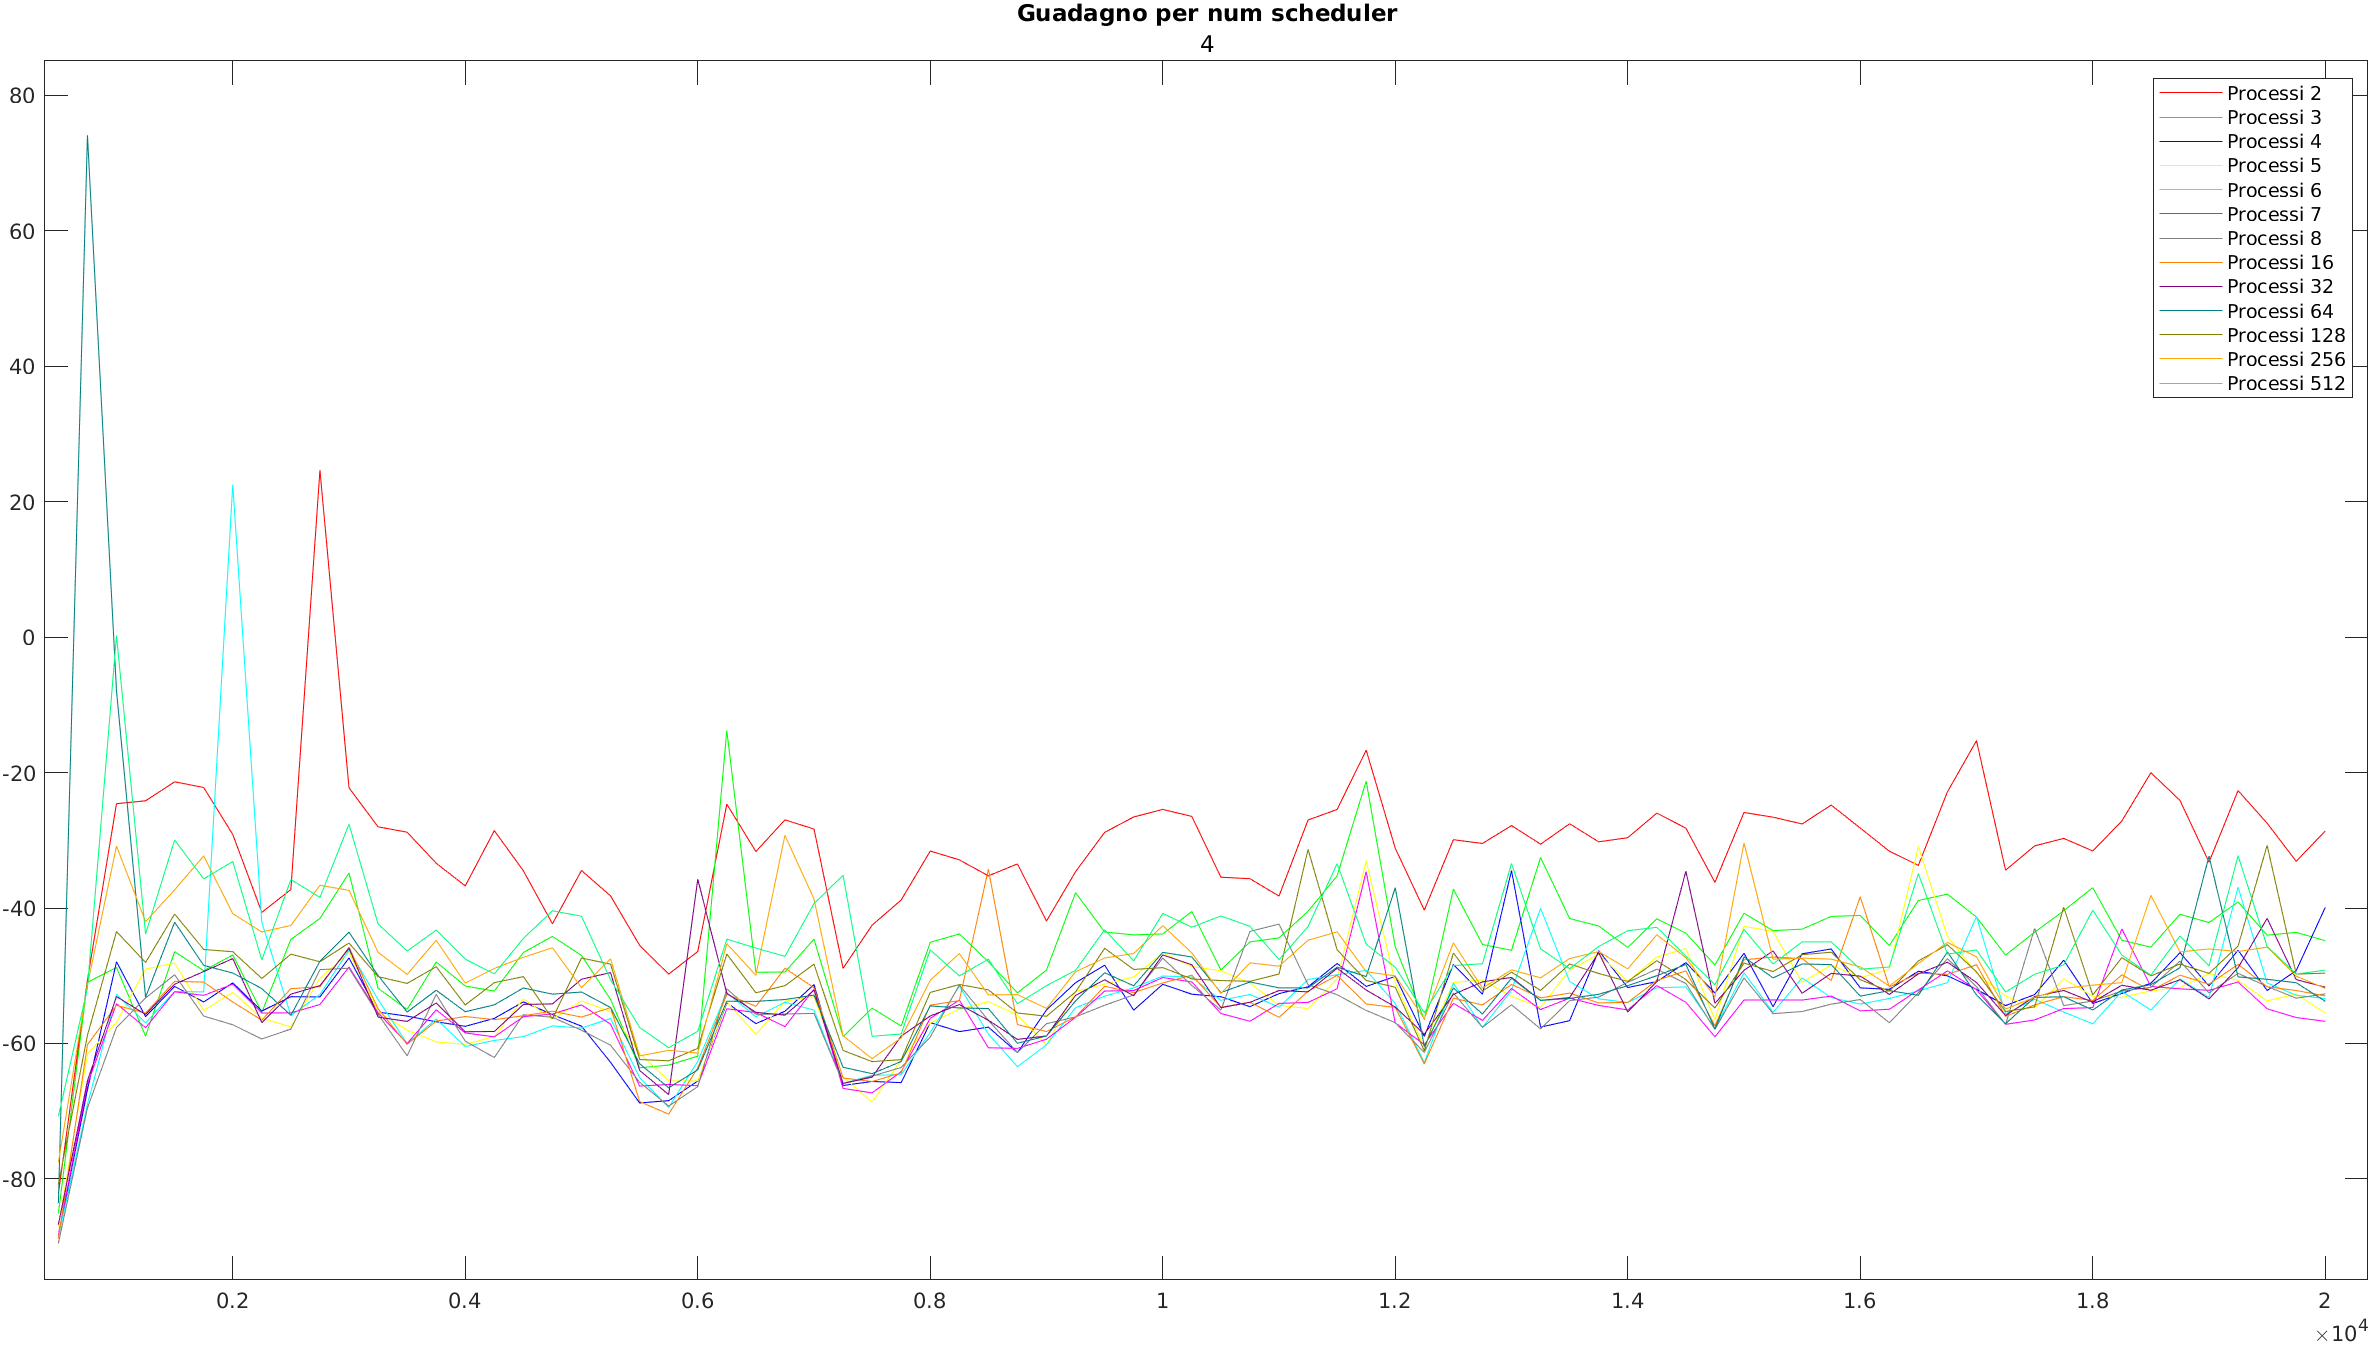
\includegraphics[keepaspectratio=true,scale=0.33]{images/matlab/io_guadagno/4_io_guadagno.png}
	\caption{Guadagno rispetto a 1 processo con 4 scheduler}
  	\label{fig:4_io_guadagno}
\end{figure}

\begin{figure}[!htp]
    \centering
    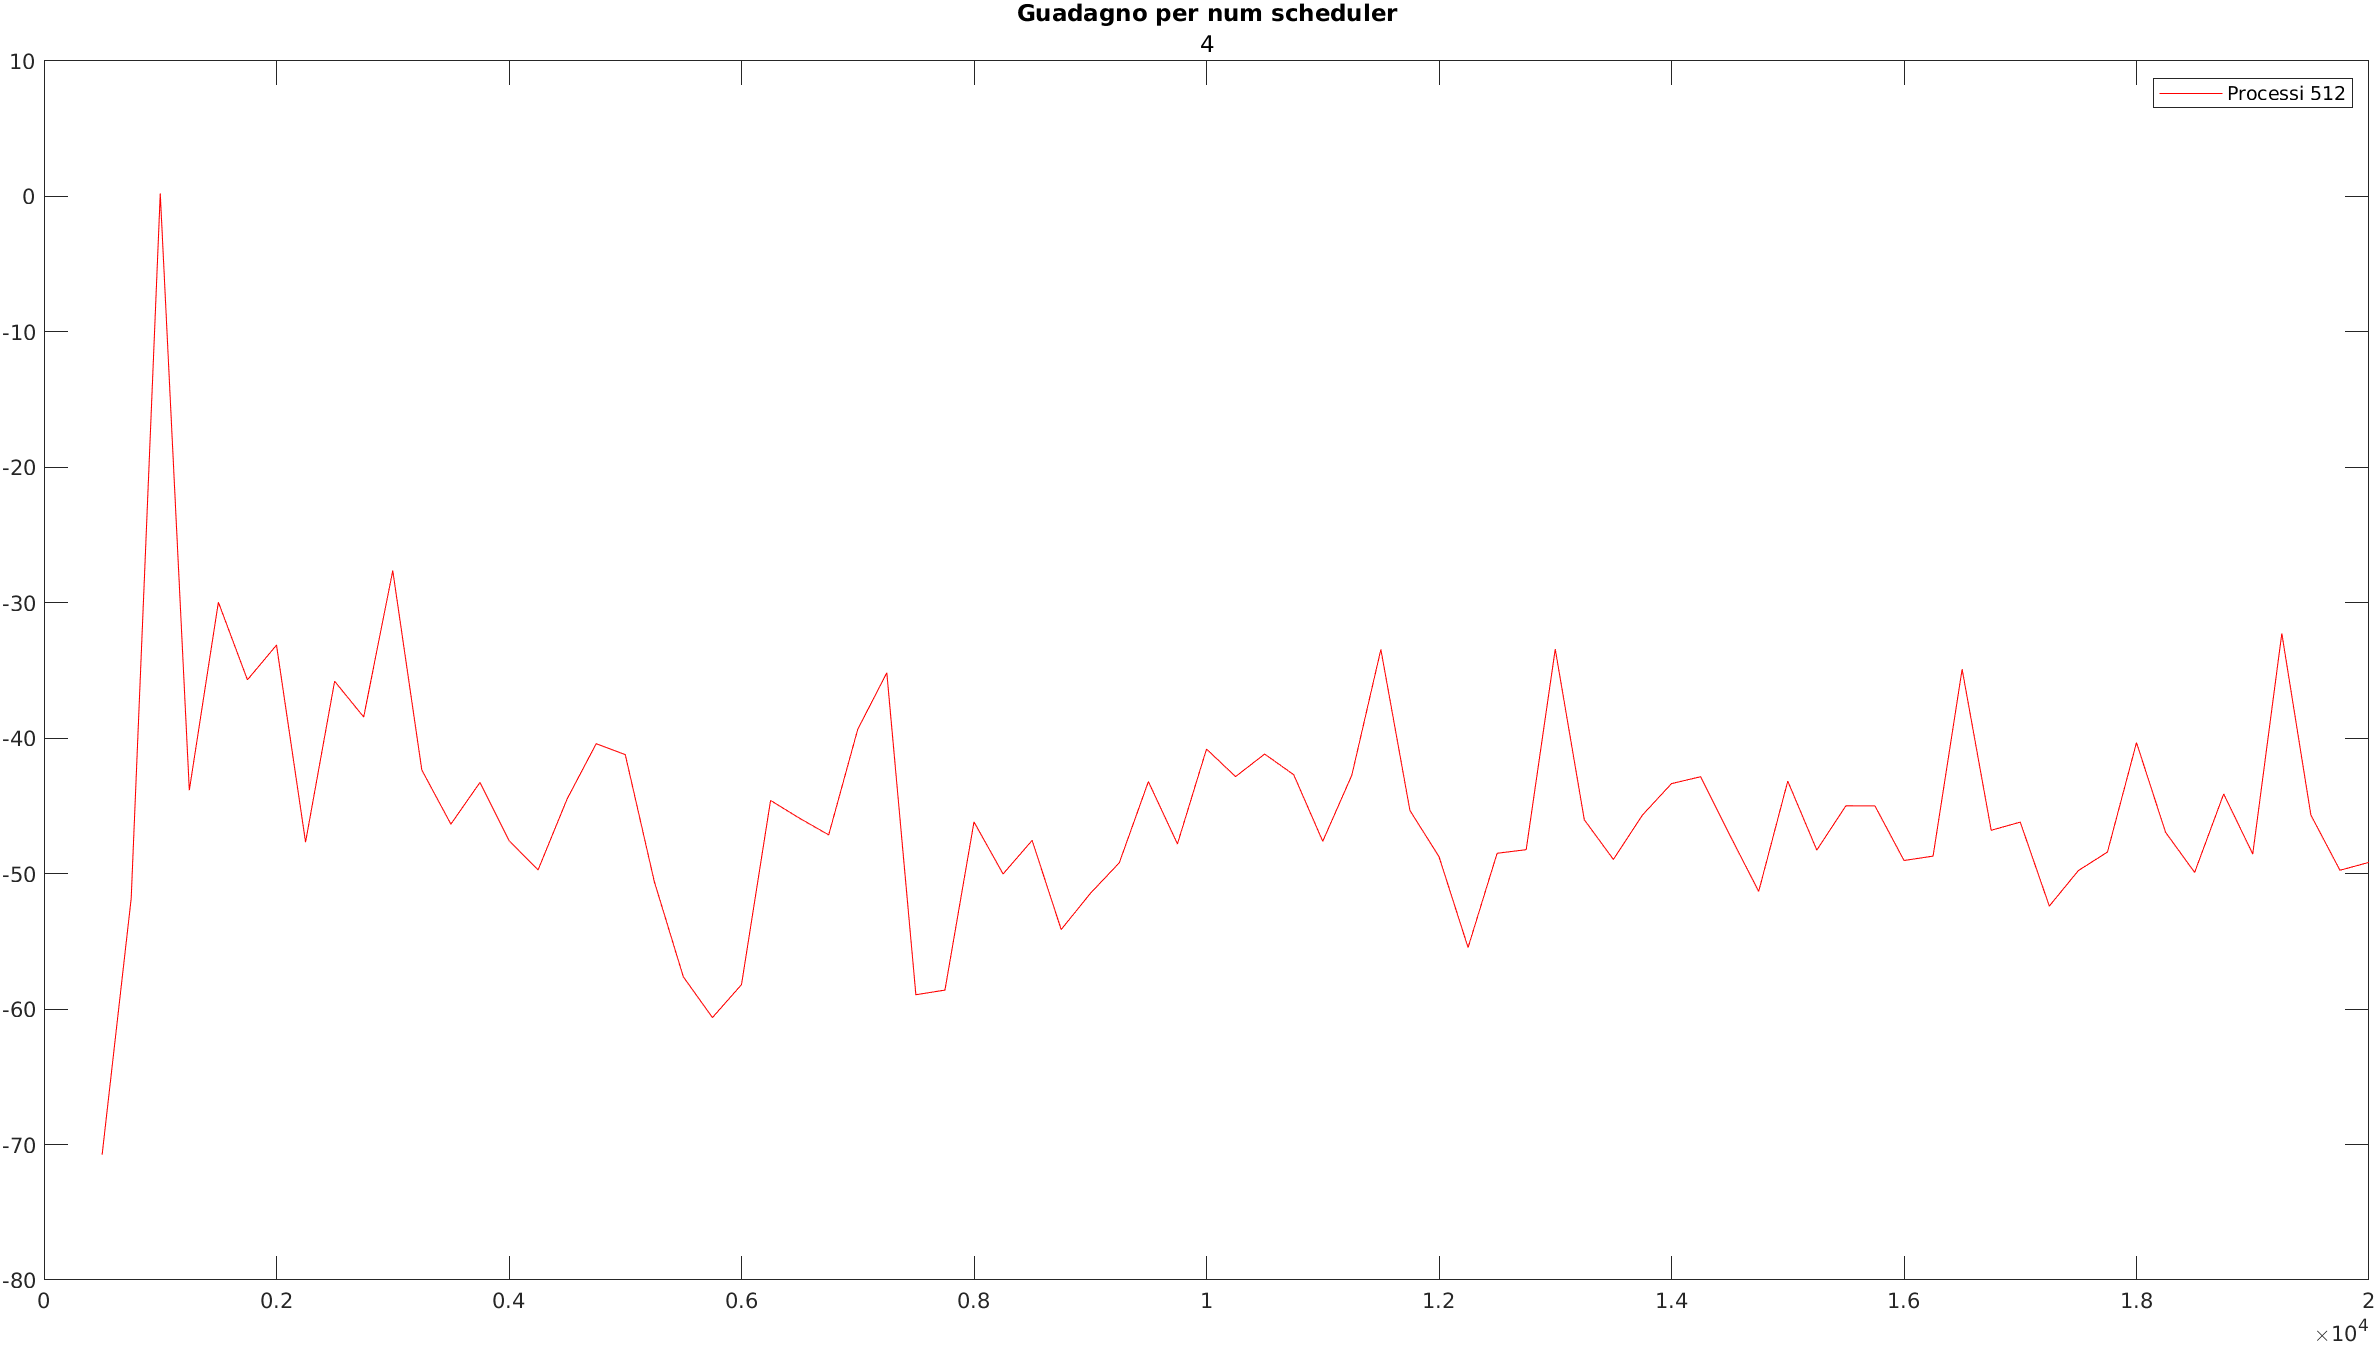
\includegraphics[keepaspectratio=true,scale=0.33]{images/matlab/io_guadagno/4_512_io_guadagno.png}
	\caption{Guadagno di 512 processi rispetto a 1 processo con 4 scheduler}
  	\label{fig:4_512_io_guadagno}
\end{figure}
